\documentclass{standalone}
\usepackage{tikz}
\usetikzlibrary{shapes.geometric,decorations.markings,arrows,positioning}

\tikzset{
    buffer/.style={
        draw,
        regular polygon,
        regular polygon sides=3,
        node distance=3cm,
        minimum height=6em
    }
}

\begin{document}
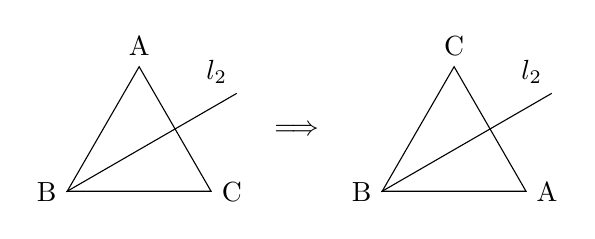
\begin{tikzpicture}
  \node[buffer] (T) {};
  \node at (T.corner 1) [above]{A};
  \node at (T.corner 2) [left]{B};
  \node at (T.corner 3) [right]{C};
  \draw (T.corner 2) -- ++(30:2.5cm) node[above left] {$l_2$};

  \node at (2,0.25) (Arr) {$\Longrightarrow$};

  \begin{scope}[xshift=4cm];
    \node[buffer] (T1) {};
    \node at (T1.corner 1) [above] {C};
    \node at (T1.corner 2) [left] {B};
    \node at (T1.corner 3) [right] {A};
    \draw (T1.corner 2) -- ++(30:2.5cm) node[above left] {$l_2$};
  \end{scope}

\end{tikzpicture}
\end{document}
